%%%%%%%%%%%%%%%%%%%%%%%%%%%%%%%
%   Mathematische Ausdrücke   %
%%%%%%%%%%%%%%%%%%%%%%%%%%%%%%%

%%%Integrale
%Integral von 0 bis pi/2
\renewcommand{\intpihalbe}{\int_{0}^{\frac{\pi}{2}}}
\renewcommand{\intnullbisn}{\int_{0}^{n}}
\renewcommand{\inteinsbisn}{\int_{1}^{n}}

%%%Summen
\renewcommand{\summeeinsbisn}{\sum_{i = 1}^{n}}
\renewcommand{\summeeinsbisnpluseins}{\sum_{i = 1}^{n+1}}
\renewcommand{\summenullbisn}{\sum_{i = 0}^{n}}
\renewcommand{\summenullbisnpluseins}{\sum_{i = 0}^{n+1}}

%%%Produkte
\renewcommand{\produkteinsbisn}{\Pi_{i=1}^{n}}
\renewcommand{\produkteinsbisnpluseins}{\Pi_{i=1}^{n+1}}
\renewcommand{\produktnullbisn}{\Pi_{i=0}^{n}}
\renewcommand{\produktnullbisnpluseins}{\Pi_{i=0}^{n+1}}

%%%Limes
\renewcommand{\limesngegenunendlich}{\lim_{n \rightarrow \infty}}
\renewcommand{\limesngegenminusunendlich}{\lim_{n \rightarrow - \infty}}
\renewcommand{\limesxgegenunendlich}{\lim_{x \rightarrow \infty}}
\renewcommand{\limesxgegenminusunendlich}{\lim_{x \rightarrow - \infty}}

%%%%%%%%%%%%%%%%%%%%%%%%%%%%%%%%%%%%%%
%   Umrandungen um Matheausdruecke   %
%%%%%%%%%%%%%%%%%%%%%%%%%%%%%%%%%%%%%%

%Schwarzer Kasten um Ausdruck => Es muss $formel$ angegeben werden
\renewcommand*{\rectangled}[1]{\tikz[baseline=(char.base)]{
\node[shape=rectangle,draw,inner sep=2pt] (char){#1};}}
%Roter Kasten um Ausdruck => Es muss $formel$ angegeben werden
\renewcommand*{\redrectangled}[1]{\tikz[baseline=(char.base)]{
\node[shape=rectangle,draw,inner sep=2pt, red] (char) {\textcolor{black}{#1}};}}
%Schwarzer Kreis um Ausdruck => Es muss $formel$ angegeben werden
\renewcommand*\circled[1]{\tikz[baseline=(char.base)]{
\node[shape=circle,draw,inner sep=1pt] (char) {#1};}}
%Roter Kreis um Ausdruck => Es muss $formel$ angegeben werden
\renewcommand*\redcircled[1]{\tikz[baseline=(char.base)]{
\node[shape=circle,draw,inner sep=1pt] (char) {\textcolor{red}{#1}};}}

%%%%%%%%%%%%%%%%%%%%%%%%%%%%%%%%%%%%%%%%%%%%%%%%%%%%%%%%%%%
%%%%%%%%%%%%%%%%%%%%%%%%%%%%%%%
%   Neue nützliche Commands   %
%%%%%%%%%%%%%%%%%%%%%%%%%%%%%%%
\renewcommand{\liste}[2]{
{\renewcommand{\arraystretch}{1.5}
\begin{tabular}{*#1{|c}|}
    \hline
    #2\\\hline
\end{tabular}}
}

%%%%%%%%%%%%%%%%%%%%%%%%%%%%%%%%%%%%%%%%%%%%%%%%%%%%%%%%%%%
\subsection{Die Registermaschine}
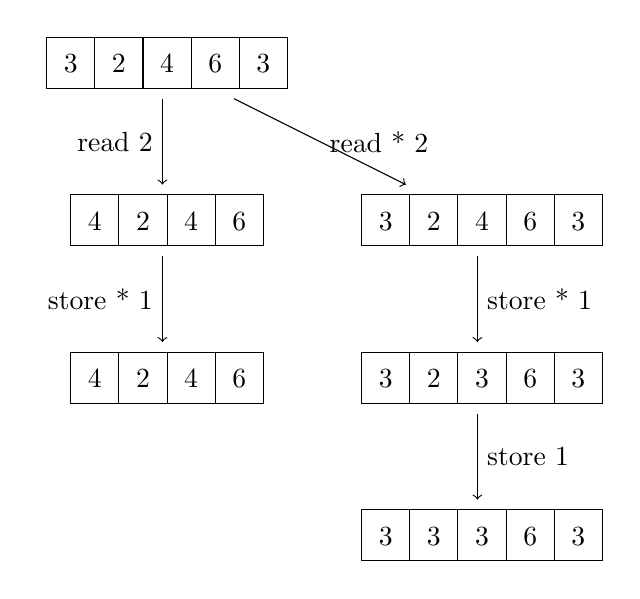
\begin{tikzpicture}
\node (1) at (0, 0) [] {\liste{5}{3 & 2 & 4 & 6 & 3}};
\node(2) at (0, -2) [] {\liste{4}{4 & 2 & 4 & 6}};
\node(3) at (4, -2) [] {\liste{5}{3 & 2 & 4 & 6 & 3}};
\node (4) at (0, -4) [] {\liste{4}{4 & 2 & 4 & 6}};
\node (5) at (4, -4) [] {\liste{5}{3 & 2 & 3 & 6 & 3}};
\node (6) at (4, -6) [] {\liste{5}{3 & 3 & 3 & 6 & 3}};
\draw[->] (1) to node[left]{read 2} (2);
\draw[->] (1) to node[right]{read * 2} (3);
\draw[->] (2) to node[left]{store * 1} (4);
\draw[->] (3) to node[right]{store * 1} (5);
\draw[->] (5) to node[right]{store 1} (6);
\end{tikzpicture}

\subsubsection{Beispiel für jump}

\begin{verbatim}
    1 | store 2
    2 | load k
    3 | jzero 9
    4 | add -1
    5 | store 1
    6 | load 2 (später read 2)
    7 | add 1
    8 | jump 3
    9 | halt
\end{verbatim}

Für $k$ setzen wir mal 3 ein.
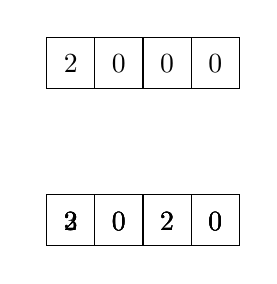
\begin{tikzpicture}
\node (0) at (0,0) []{\liste{4}{2 & 0 & 0 & 0}};
\node (1) at (0,-2) []{\liste{4}{2 & 0 & 2 & 0}};
\node (1) at (0,-2) []{\liste{4}{3 & 0 & 2 & 0}};
\node (1) at (0,-2) []{\liste{4}{2 & 0 & 2 & 0}};
\node (1) at (0,-2) []{\liste{4}{2 & 0 & 2 & 0}};
\end{tikzpicture}

{\renewcommand{\arraystretch}{2}
\begin{tabular}{c|l}
     Registermaschine & Zähler\\\hline
     \liste{5}{$r_0$ & $r_1$ & $r_2$ & $r_3$ & ...}&\\
     \liste{5}{2 & 0 & 0 & 0 & ...} & t = 0 (Programmstart)\\
     \liste{5}{2 & 0 & 2 & 0 & ...} & z = 1\\
     \liste{5}{3 & 0 & 2 & 0 & ...} & z = 2\\
     \liste{5}{2 & 0 & 2 & 0 & ...} & z = $\not 3 \ 4$\\
     \liste{5}{2 & 2 & 2 & 0 & ...} & z = 5\\
     \liste{5}{2 & 2 & 2 & 0 & ...} & z = 6\\
     \liste{5}{3 & 2 & 2 & 0 & ...} & z = 7\\
     \liste{5}{3 & 2 & 2 & 0 & ...} & z = 8\\
     \liste{5}{3 & 2 & 2 & 0 & ...} & $z = 3 \Rightarrow 4$\\
     \liste{5}{2 & 0 & 0 & 0 & ...} & \\
\end{tabular}}

\begin{align*}
    r_0 = r_0 + r_j
\end{align*}

\begin{verbatim}
    while r_j > 0
        r_0 = r_0 + 1
        r_j  --
\end{verbatim}

Die Laufzeit beträgt normal: $O(r_j)$

\subsection{Effiziente Algorithmen}

\newcommand{\tcal}{\mathcal{T}_{\mathcal{M}}}
\begin{align*}
    \mathcal{T}_M(e) &= \begin{cases}
    |e| & \text{, wenn } e \text{ gerade}\\
    c & \text{, sonst}
    \end{cases}\\
    &= \tcal(n) = \max\{\tcal (e) \log_2(2 + |e|) \leq n\}\\
    &= O(2^n)\\
    &\max \{\tcal(2^k)| k \leq n\}\\
    &= \max \{\tcal(2^n), \tcal(2^{n-1})\}\\
    &= O(2^n)
\end{align*}
Länge $n$ größte $e$ $|e|= 2^{n-1}$\\
$\Rightarrow$ Maximum aller $e$ mit $|e| \leq 2^n$\\

\begin{tabular}{cccc}
    &mit Addition & ohne Addition & mit Muliplikation\\
    $r_0 = r_0 + r_j$&$O(1)$ & $O(|r_j|)$\\
    $r_0 = r_0 * r_j$&$O(|r_j| \cdot r_j|)$ & & $O(1)$ 
\end{tabular}

n-mal $r_0 * r_0$ $2^{2^n}$
\begin{align*}
\begin{cases}
\text{mult-Befehl:} & O(n)\\
\text{add } r_j & O(2^n) \rightarrow\text{ exponentieller Unterschied zu mult-Befehl}
\end{cases}
\end{align*}
